\chapter{Introduction}

In this research we explored various optimization techniques based on programming features. Initially this research started with idea of finding optimal web server architecture based on programming features of Ballerina language. With extensive tuning of Ballerina's internal architecture it was able to identify tuning the thread pool size of the existing architecture is the best way maximize the performance for given set of programming features.

\section{Background to the Research}

Web server optimization is prominent branch in the enterprise level software industry. Optimization aids to utilize the resources efficiently for web servers. This research came along long way and narrowed down from web server architecture implementation to thread pool optimization using programming features in Ballerina language. Prior determination of web sever architecture that perform best is difficult due to various factors such as type of workload that process, working environment \cite{comp_ac} etc. It is challenging to provide the best architecture for all type of workload \cite{seda,events_are_bad,edprs} because implementation of framework and language affect the performance as well.Also, there is no knowing mechanism to identify the type of workload prior to the execution of program and selecting best web server architecture for identified workload. 

\newpage

\section{Research Problem and Research Questions}\label{sec:research_questions}

This research addresses the following questions.


\begin{itemize}
	
  	%\item What are the parameters required to tune in Ballerina's internal server architecture to maximize the performance for a given program type?
 	%\item Is it possible to propose optimal web server architecture or parameters based on program features?
 	
 	\item Can we find a server architecture and parameters that would result in the best performance for a given Ballerina program? 
 	\item Can we tune the thread pool size of a given server architecture in order to optimize the performance (i.e. throughput and latency)? If so what is the impact of the thread pool size on the performance for different Ballerina programs? 
 	\item Can we devise a model that can estimate the thread pool size that would result in the best performance for a given Ballerina program?
\end{itemize}


%%\begin{figure}[htbp]
%%  \begin{center}
%%    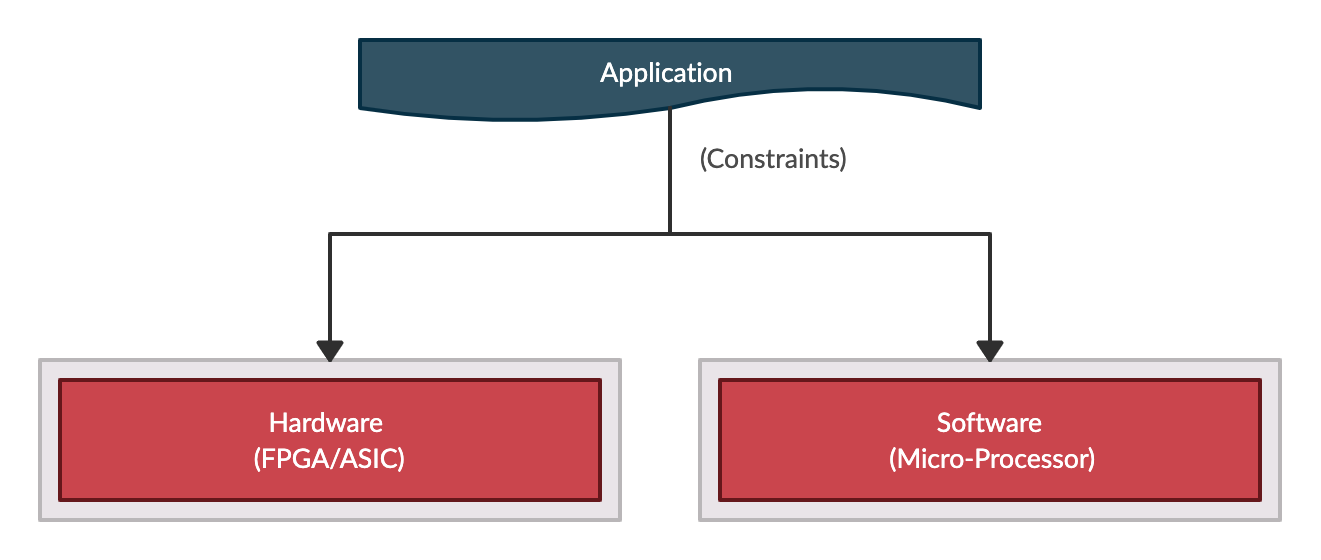
\includegraphics[scale=0.3]{images/problem.png}
%%    \end{center}
%%  \caption{HW/SW Paritioning problem}
%%\end{figure}


\section{Justification for the research}

 In the previous researches, they tried to provide optimal web server architecture for offered workload. Also, there is no global model to generalize the findings of those researches. This research tries to find model to predict optimal web server architecture for given program for the Ballerina language which is designed for network programming.  Also, there are a number of researches for thread pool tuning with black box and white box approaches. All approaches have their own advantages and disadvantages. This research proposes technique using machine learning to find optimal thread pool size for given program.  
 
 None of previous researches have been automated the identification of programming features automatically and propose the web server architecture or optimal thread pool size for given set of features or user programs. Ballerina is a better candidate for the research because identification of the programming features is more convenient in Ballerina. Features that are harder to extract in other languages are part of the Ballerina language.  


\section{Methodology}

	This research started with implementing new web sever architectures in Ballerina and then evaluating the performance of each including the existing architecture (Look figure \ref{bal_internal}). These architectures are inspired from Thread per connection model and event based models(Ex: \acrshort{seda}). This step includes modifying the Ballerina source code. Proper implementation requires deep analysis of Ballerina run time and optimization for the implementations, otherwise bugs can affect the performance. 
	
	Performance are evaluated with test programs which consist of different programming features. As an example one program may consists of several database calls and another program only contain the some arithmetic operations. Then performance are evaluated according to program features. The target is to provide best performant architecture for given features. Fine-tunes are carried out based on results of each phase. That led the research to focus on thread pool tuning after number of experiments. 
	
	Final model is consisted of a machine learning model that provide optimal thread pool size for given program. Figure  \ref{hl_architecture} shows the overview of the research. Results are dependent of the deployment environment of the service. Hence, first user need to train the machine learning model with predefined set of programs. The user able to provide own program and the model predict the optimal thread pool size for that program. These steps are explained more detail in Chapter 3.   
	
	\begin{figure}[htbp]
		\begin{center}
			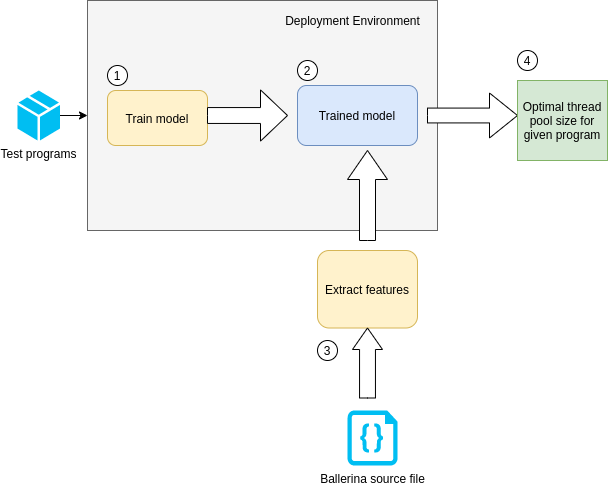
\includegraphics[scale=0.5]{figures/hl_architecture.png}
		\end{center}
		\caption{High-level overview of the research}
		\label{hl_architecture}
	\end{figure}
	

\section{Outline of the Dissertation}

This dissertation outlines 6 chapters as follows.

\begin{enumerate}
	\item Introduction
	\item Literature Review 
	\item Research Design
	\item Implementation
	\item Results \& Evaluation — Contain the results obtained in each phase and in depth discussion of the results.
	\item Conclusion — Discuss how the results mentioned in Chapter 5 has addressed the research questions. An emphasis will be given in highlighting the contribution of this research work to the scientific world. Implications of further research will also be discussed in this chapter.
\end{enumerate}

\section{Definitions}

\subsubsection{Concurrency level}

In this research Concurrency level and Concurrency users are used interchangeably referred to concurrent users who are connected the web server. This value can be  simulated in load testing software. A good web server must be able to perform well in higher number of concurrency level.

\subsubsection{Deployment environment}

Deployment environment is where web server is deployed and running. Configuration of the environment includes the Operating system, Number of CPU core, Speed of the CPU, Amount of RAM and Network stability etc.

\subsubsection{Server architecture}

%Results are subjects to the configurations of that environment.

\section{Delimitations of Scope}

\subsection{In-Scope}

\begin{itemize}
	\item Implement new server architectures in Ballerina by modifying the existing implementation. This includes adding and removing new thread pools. Then performance is evaluated using relevant metrics .
	\item Fine tune and optimize the new architectures by identifying bugs and debugging — these tuning includes the changing thread pool size.
\end{itemize}

\subsection{Out-Scope}

\begin{itemize}
	\item Generalizing the findings for other languages and frameworks
	\item Evaluate and compare the model for different deployment environments.
	\item Design and implementation of analytical (aka white box model in this research) model (using queuing theory etc. ) to predict optimal thread pool size.
\end{itemize}

\section{Conclusion}	

This chapter provides base principles and presents a foundation to the dissertation. At the beginning, the research problem is identified, formulated research questions, and research is justified. Then the definitions is presented, dissertation is outlined, research design and implementation is briefly discussed laying the path to proceed with detailed explanation of the research.